%%\documentclass[sigconf, nonacm]{acmart}
%%\documentclass{article}
\documentclass[13pt,english]{article}
\usepackage[T1]{fontenc}
\usepackage{babel}
\AtBeginDocument{%
  \providecommand\BibTeX{{%
    \normalfont B\kern-0.5em{\scshape i\kern-0.25em b}\kern-0.8em\TeX}}}

\usepackage{url}
\usepackage{graphicx} %package to manage images
\graphicspath{ {./images/} }
\usepackage[utf8]{inputenc}
\usepackage{hyperxmp}
\usepackage{fancyhdr}
\pagestyle{fancy}
\usepackage{lipsum}
\usepackage{caption}
\usepackage{subcaption}
\pagenumbering{roman}
\usepackage{hyperref}
\hypersetup{
    colorlinks=true,
    linkcolor=blue,
    filecolor=magenta,      
    urlcolor=blue,
    pdftitle={Overleaf Example},
    pdfpagemode=FullScreen,
    }

\begin{document}

\title{TP3 Homework Submission}
\date{February 22, 2022}

\author{
  Vincent, Wilmet\\
  \texttt{vincent.wilmet@student-cs.fr}
  } 

\maketitle

\section{{Graph Neural Networks}}
We are given a basic Graph Convolutional and the Protein-Protein Interaction (PPI) network dataset for benchmarking. One graph of the PPI dataset has on average 2372 nodes. This multilabel classification problem has 121 gene ontology sets (way to classify gene products like proteins) that must be classified using 50 features (positional gene sets / motif gene / immunological signatures, etc).

\subsection{Training Process, Hyperparameters and GridSearch}
Initially, without any modifications to the given code, the model performs very poorly. Although it doesn't gives NaN values, nor errors, the model reaches an average F1 score of 0.51 on 20 trials. \\

With this in mind, I decided preprocess the data for better model performance. I did this by trying sklearn methods like MinMaxScaler, StandardScaler and normalize with l1, l2, and max norms. This later showed to be unhelpful with larger models. Furthermore, after reading the papers describing the PPI dataset published by Stanford computational neuroscientists, I understood I was far out of my domain of expertise and if they curated the dataset to be a certain way, it should stay a certain way. At least until I learned what is malleable. \\

The following hyperparameters are applied to this problem. Because GridSearch is not implemented in PyTorch, I used a very oldschool technique: nested for-loops for each of the hyper-parameters listed above. I used early stopping to avoid time wasted training on a poorly performing model. \\
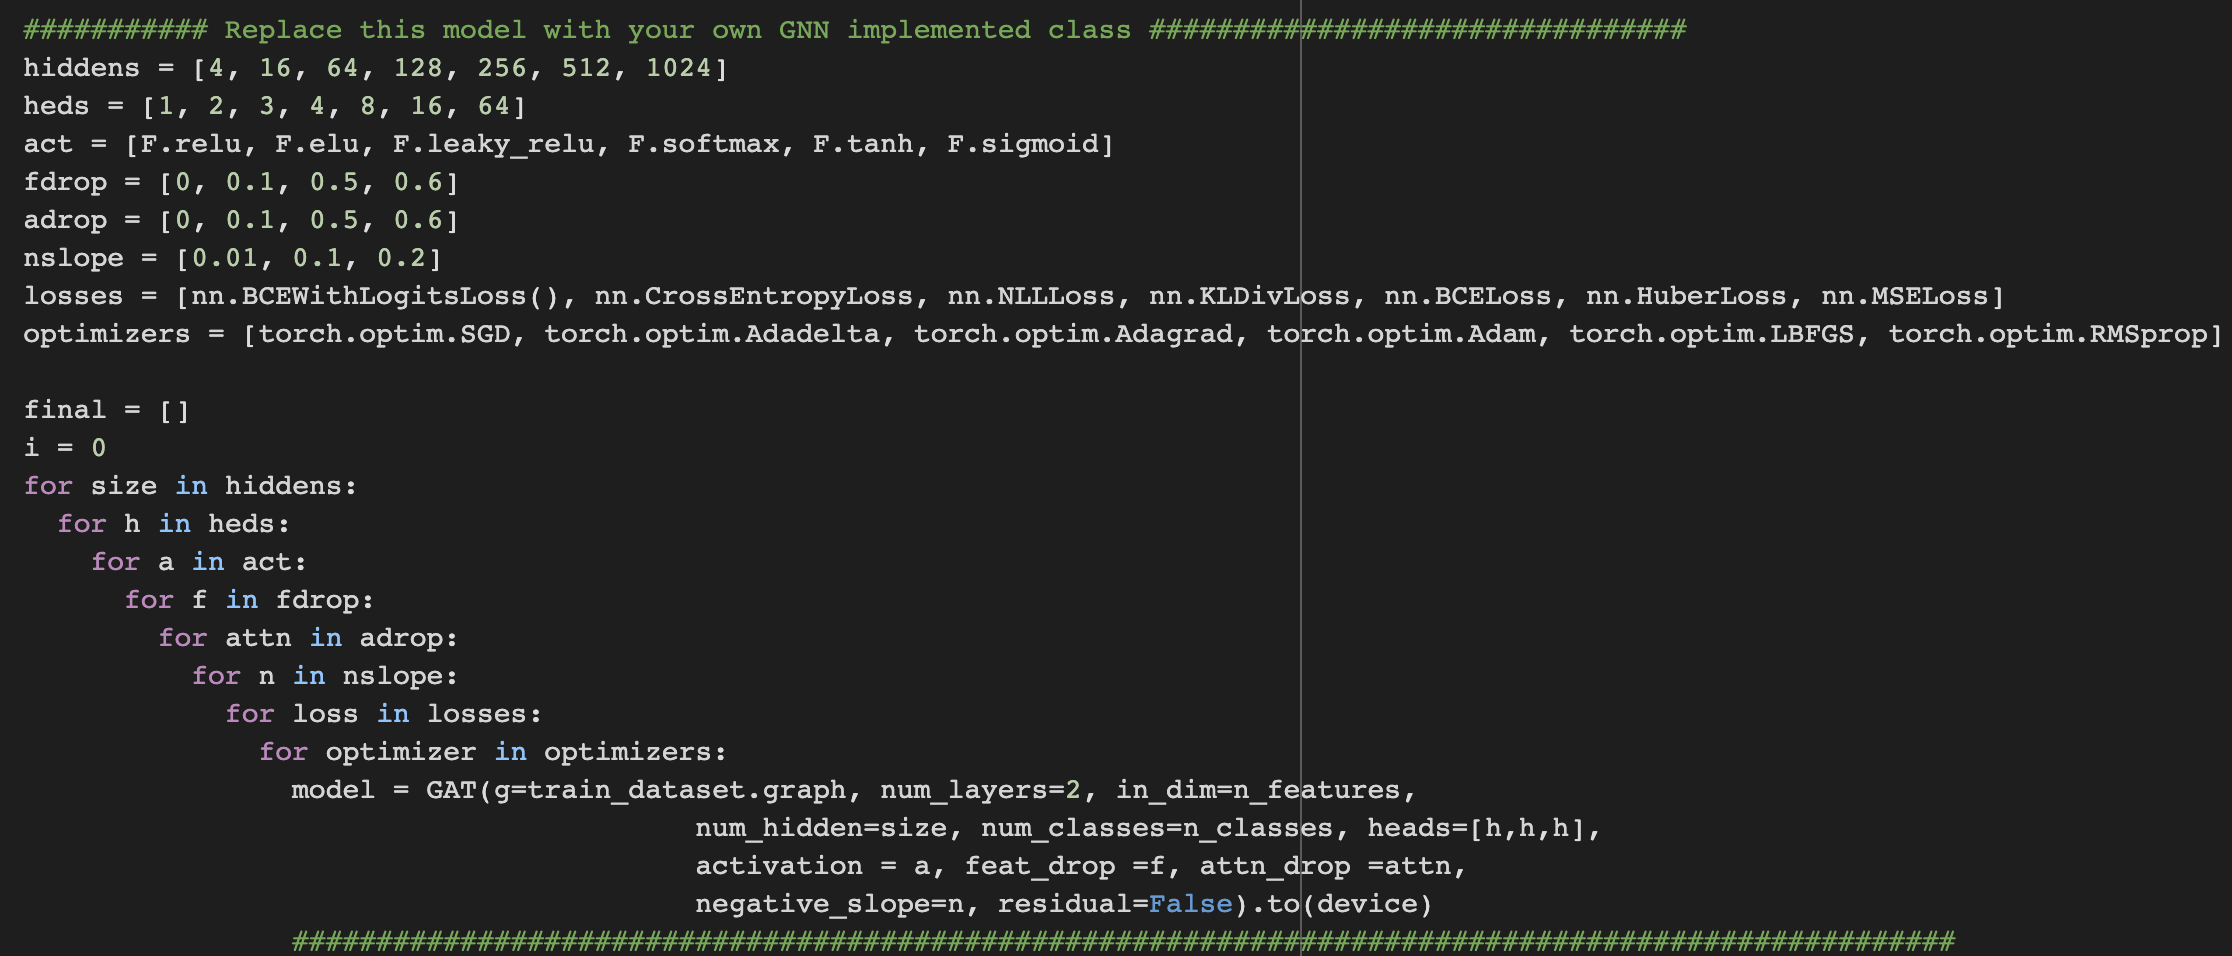
\includegraphics[width=\textwidth]{hyperparameters.png} \\

In all there are 7*7*6*4*4*3*7*6=592,704 possible configurations. Of course, after nearly 30 hours, I had exceeded the monthly allocation for Google Colab's GPUs and I understood that doing all combinations would be infeasible. It was taking about 0-4 minutes to run each model depending if it stopped at 10, 50, 100, 150 or 250 epochs. \\
I tried a variation of each non-numeric parameters (activation functions, loss functions and optimizers) to find that the best activation functions were ReLU and eLu, loss functions limited to BCEWithLogitsLoss and MultiLabelSoftMarginLossm and only Adam for optimizer. Everything else either crashed or rarely surpassed a 60\% F1 score. AdaGrad did surprisingly well, and CrossEntropyLoss was surprisingly poor performing. I learned that the high drop out rates would do well in the beginning of training but cause the model to be erratic by the end of 250 epochs. And as much as I think 16+ heads and 1024 hidden layers would make the model perform better, Colab could not handle the size of the models loaded to memory. \\
After limiting the configurations, I received the following results for best performing models. Unsurprisingly, the ones with highest head size and hidden layers top the list. \\
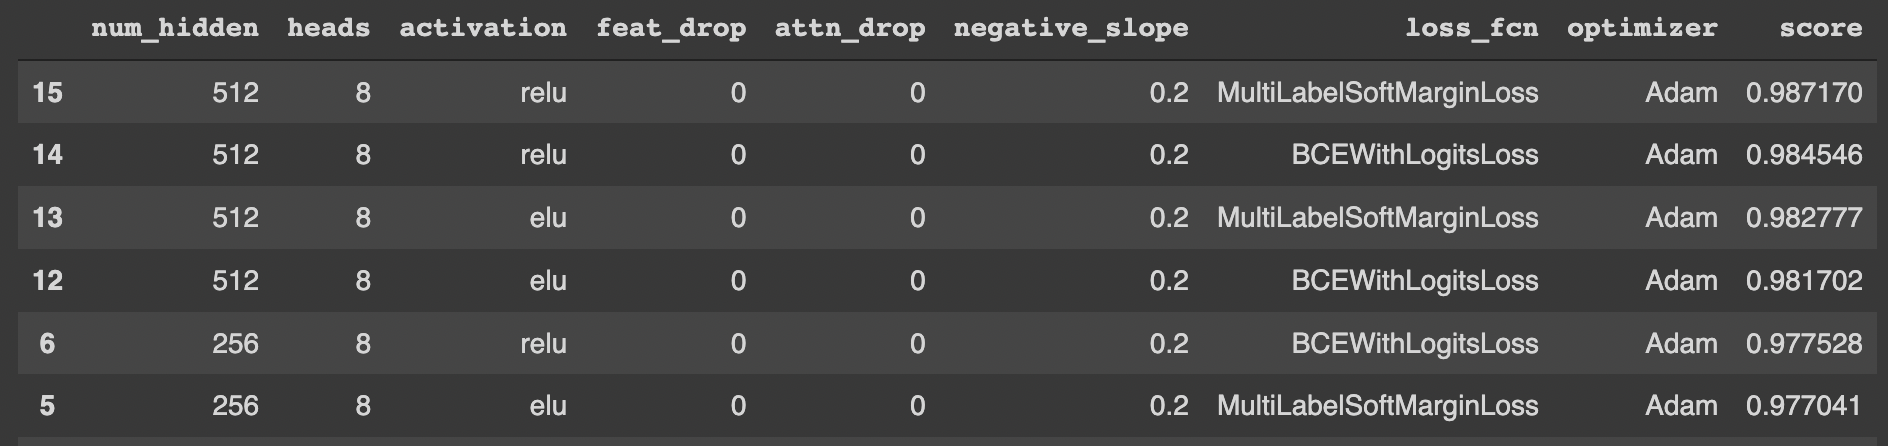
\includegraphics[width=\textwidth]{sorted.png} \\

\subsection{Model Architecture}
The final model uses the following hyperparameters:
\begin{verbatim} 
hiddens = [512]
heds = [8] 
activations = [F.relu]
fdrop = [0]
adrop = [0]
nslope = [0.2]
losses = [nn.MultiLabelSoftMarginLoss()]
optimizers = [torch.optim.Adam]
\end{verbatim}
and looks like this: \\
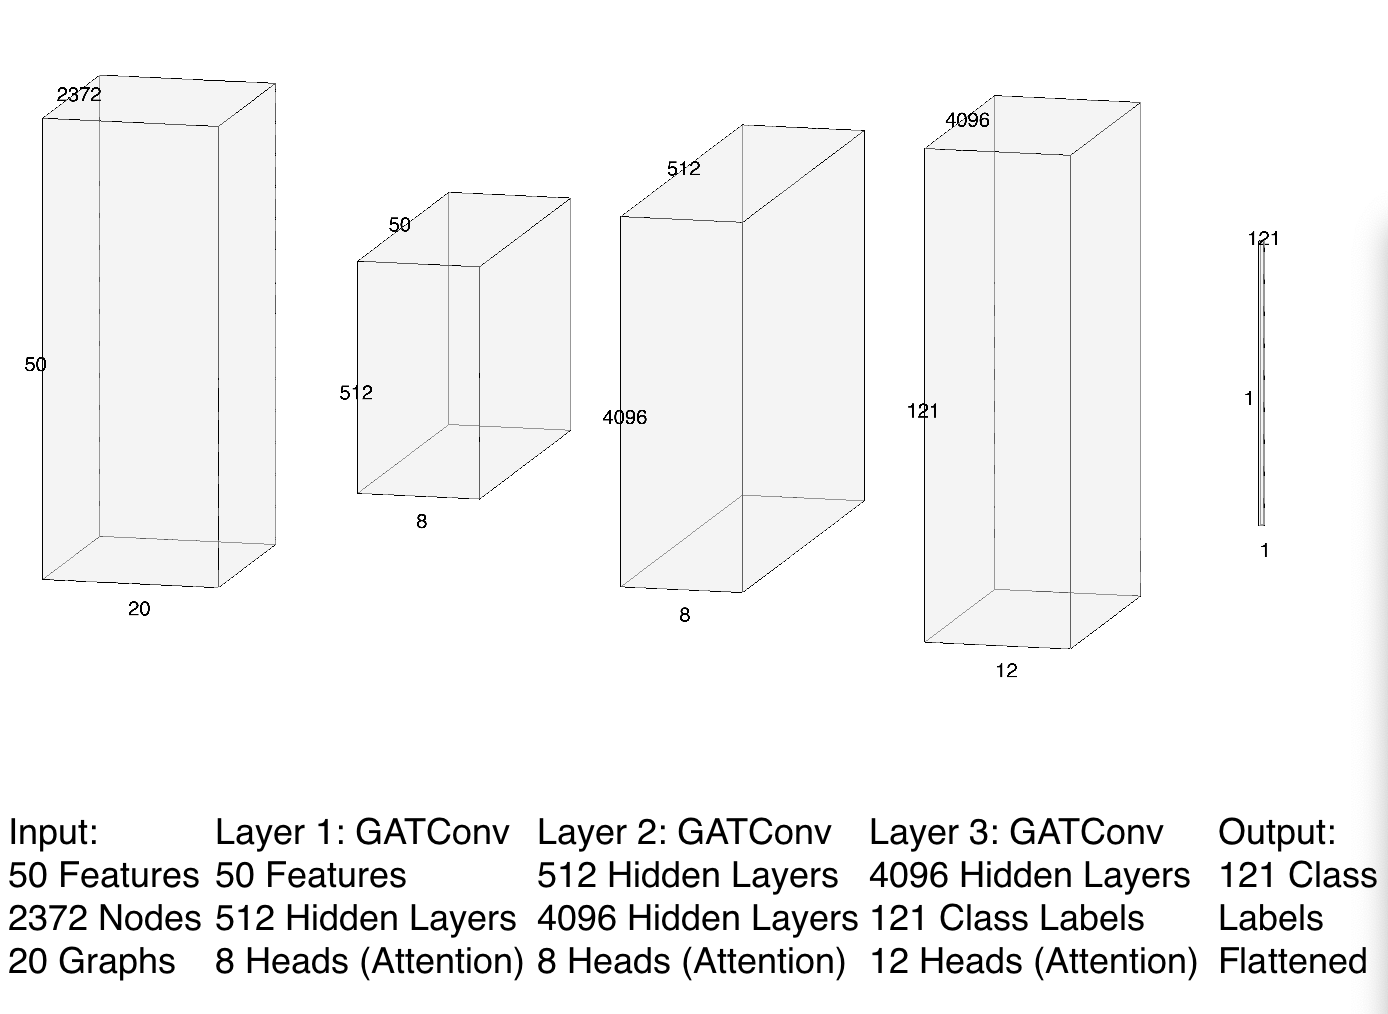
\includegraphics[width=\textwidth]{architecture.png} \\
The below graph shows the GAT attention module in detail as described by the original authors Velickovic et al in their 2018 paper \href{https://arxiv.org/pdf/1710.10903.pdf}{GRAPH ATTENTION NETWORKS}. \\
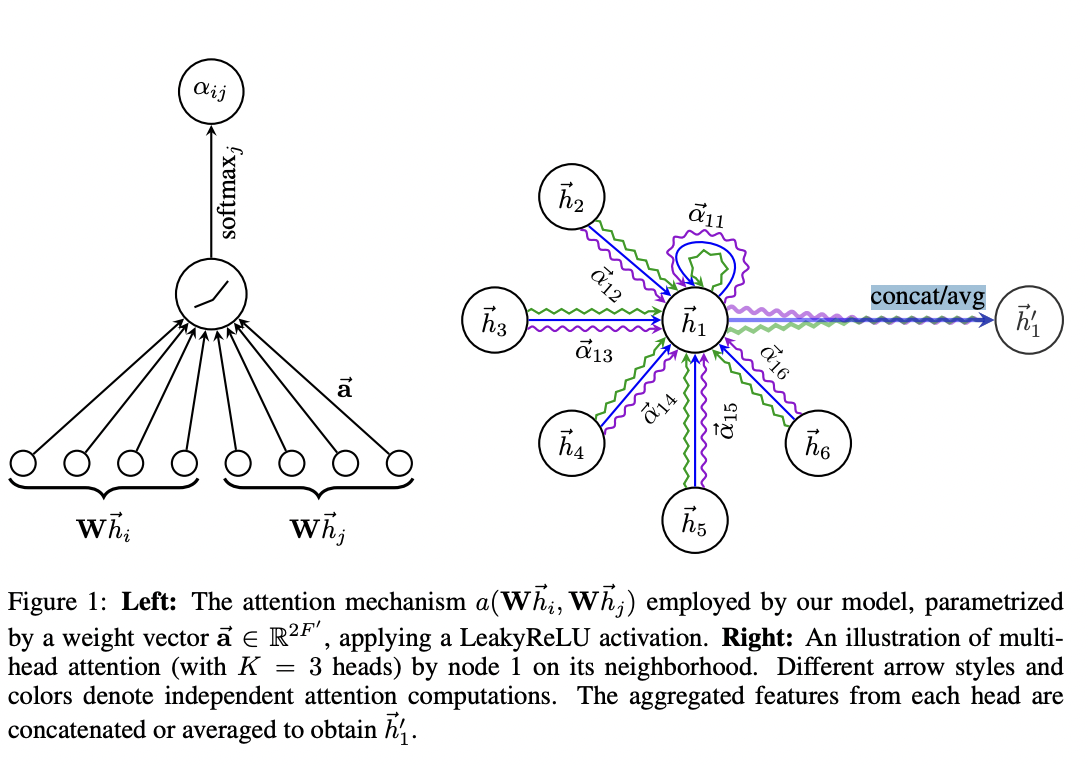
\includegraphics[width=\textwidth]{attention.png}


\subsection{Performance and Results}
Ultimately, the best performing model reached heights of 0.9956994061645773, but on an average of 20 trials had an \textbf{F1 Score of 0.9865}. The reason it is not consistent, even though the GATConv uses a uniform Xavier initializer for its weights, is the Adam optimizer starts in a random corner each time the model is trained. \\
We can see that it vastly out performs the baseline model, which rarely surpassed a F1 Score of 0.50 on multiple trials. This is because multi-headed Graph Attention models are able to capture the relationships between the Protein-Protein Interactions (PPI) much better than a Convolutional network can. 

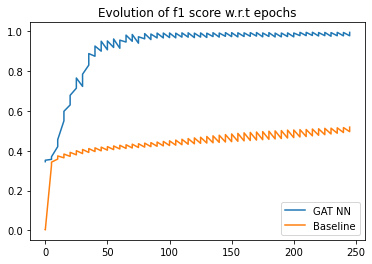
\includegraphics[width=\textwidth]{F1Scores.png} \\


What we can learn from this model is that the Graph Attention model uses an "attention" mechanism to focus on the most important nodes within the graph network. They do this by assigning larger weights to more important nodes, which are found by looking at the relative weights between two neighboring connected nodes. \\
This is in contrast to the Graph Convolutional model which reassigns its attention weights in every walk. This makes the weights between each connected pair different for each layer and thus the mutual dependencies are a lot harder to identify. \\
GAT models, on the other hand, rapidly enhances the rate at which important nodes are identified and learned, at the expense of computing for each node combination.  
\end{document}
